%(BEGIN_QUESTION)
% Copyright 2010, Tony R. Kuphaldt, released under the Creative Commons Attribution License (v 1.0)
% This means you may do almost anything with this work of mine, so long as you give me proper credit

\noindent
{\bf Programmeringsutfordring -- pumpevalg med utjevning av driftstid}

\vskip 10pt

I kritiske prosessapplikasjoner er det vanlig med to eller tre pumper der én pumpe normalt ville vært tilstrekkelig. Kommunal vannforsyning og avløpssystemer bruker ofte doble pumper for redundans: én pumpe kan overta hvis den andre feiler:

$$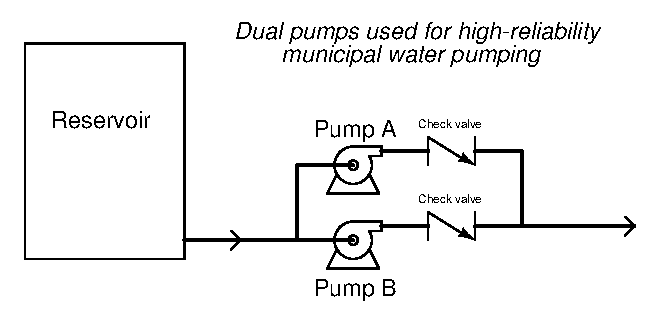
\includegraphics[width=15.5cm]{i00126x01.eps}$$

Et mulig problem med doble pumper er at «reservepumpen» kan få mekaniske problemer hvis den står stille for lenge, og dermed ikke fungerer som backup når hovedpumpen feiler. En løsning er å velge neste pumpe som skal starte basert på hvilken som har lavest akkumulert driftstid. Hver gang en pumpe skal starte, velges den med færrest driftstimer.

\vskip 10pt

Skriv et PLC-program som tar «Start»- og «Stop»-trykknappsignaler inn, og styrer to pumper på denne måten.

\vfil 

\underbar{file i00126}
\eject
%(END_QUESTION)





%(BEGIN_ANSWER)


%(END_ANSWER)





%(BEGIN_NOTES)

Jeg anbefaler sterkt at studenter lagrer alle PLC-programmer for framtidig referanse, kommenterer dem grundig og bruker filnavn som er enkle å søke opp senere.

\vskip 10pt

Jeg anbefaler også å bruke disse programmene som korte klasseoppgaver, og deretter be om skjermbilder fra studentene (via minnepinne, e-post eller annen filoverføring) når tiden er ute. Hensikten er både å få studentene aktive i PLC-programmering og å la dem se andre studenters løsninger på samme problem. Skjermbildene kan sendes tilbake til studentene ved slutten av dagen, slik at de får flere løsninger å studere videre.

%INDEX% PLC, programming challenge: run-time equalizing pump selection control
%INDEX% Process: municipal water flow control

%(END_NOTES)
